\documentclass[10.5pt,scale=1.0,t,aspectratio=169,hyperref={pdfpagelabels=false}]{beamer}


\usepackage{lipsum}
\usepackage{color}
\usepackage{amsfonts}
\usepackage{amsmath,mathtools}
\usepackage{mathrsfs}
\usepackage{array}
\usepackage{algorithm}
\usepackage{hyperref}
\usepackage[spanish,es-nodecimaldot]{babel}
\usepackage[utf8]{inputenc}
\usepackage{graphicx}
\usepackage{multicol}
\usepackage{multirow}
\usepackage{enumitem}
\usepackage[document]{ragged2e}
\usepackage[absolute,overlay]{textpos}
\textblockorigin{0mm}{0mm} 
\usefonttheme[onlymath]{serif}
\usepackage{verbatim}
\usepackage{cite}




\newenvironment{conditions}[1][where:]
{#1 \begin{tabular}[t]{>{$}l<{$} @{${}={}$} l}}
	{\end{tabular}\\[\belowdisplayskip]}


\newcolumntype{L}{>{$}l<{$}} % math-mode version of "l" column type


\newcounter{saveenumi}
\newcommand{\seti}{\setcounter{saveenumi}{\value{enumi}}}
\newcommand{\conti}{\setcounter{enumi}{\value{saveenumi}}}

\setbeamertemplate{bibliography item}{\insertbiblabel}


\hypersetup{colorlinks=true,
	linkcolor=blue,
	linktoc=all,				
	citecolor=blue,
	urlcolor=red,
	pdftitle={ELECTRONICA DIGITAL},
	pdfauthor={Santiago Rúa Pérez},
	pdfcreator={Santiago Rúa Pérez}}


\definecolor{GreenDark}{rgb}{0.0, 0.60, 0.0}
\definecolor{RedDark}{rgb}{183, 0.0, 0.0}
\definecolor{BlueDark}{rgb}{0.0, 0.0, 167}
\definecolor{BlueLight}{rgb}{0.2, 0.451, 0.517}


\graphicspath{{imag/}}

\newcommand{\Ho}{$H_{0}$}
\newcommand{\Ha}{$H_{a}$}
\newcommand{\Nota}{{\bf Nota: }}
\newcolumntype{P}[1]{>{\centering\arraybackslash}p{#1}}
\newcolumntype{M}[1]{>{\centering\arraybackslash}m{#1}}

\newcommand{\less}{<}
\newcommand{\greater}{>}


\setlength{\parindent}{1em}
\setlength{\parskip}{.6em}
\renewcommand{\baselinestretch}{.9}

%%%%    C environment    ---------------- %%%%%%%%%%%%%%%.
\usepackage{listings}
\usepackage{xcolor}
\definecolor{mGreen}{rgb}{0,0.6,0}
\definecolor{mGray}{rgb}{0.5,0.5,0.5}
\definecolor{mPurple}{rgb}{0.58,0,0.82}
\definecolor{backgroundColour}{rgb}{0.95,0.95,0.92}

\lstdefinestyle{CStyle}{
	backgroundcolor=\color{backgroundColour},   
	commentstyle=\color{mGreen},
	keywordstyle=\color{magenta},
	numberstyle=\tiny\color{mGray},
	stringstyle=\color{mPurple},
	basicstyle=\scriptsize,
	breakatwhitespace=false,         
	breaklines=true,                 
	captionpos=b,                    
	keepspaces=true,                 
	numbers=left,                    
	numbersep=5pt,                  
	showspaces=false,                
	showstringspaces=false,
	showtabs=false,                  
	tabsize=2,
	language=C
}
%%--------------------------------------------------------------------------


\title{Electrónica Digital II}   
\author{Santiago Rúa Pérez, PhD.} 
\date{\today} 

\setlength{\TPHorizModule}{\textwidth}
\setlength{\TPVertModule}{\textwidth}

\newcommand{\btVFill}{\vskip0pt plus 1filll}


\setbeamertemplate{sidebar right}{}
\setbeamertemplate{footline}
{
	\leavevmode%
	\hbox{%
		\begin{beamercolorbox}[wd=.333333\paperwidth,ht=2.25ex,dp=1ex,center]{author in head/foot}%
			\usebeamerfont{author in head/foot}\insertshortauthor
		\end{beamercolorbox}%
		\begin{beamercolorbox}[wd=.333333\paperwidth,ht=2.25ex,dp=1ex,center]{title in head/foot}%
			\usebeamerfont{title in head/foot}\insertshorttitle
	\end{beamercolorbox}}%
	\vskip0pt%
}
\makeatother

\begin{document}
%%%%%%%%%%%%%%%%%% FRAME %%%%%%%%%%%%%%%%%%%%%%%%%%
\begin{frame}
	\titlepage
\end{frame}
%%%%%%%%%%%%%%%%% FRAME START %%%%%%%%%%%%%%%%%%%%%%%%%%
\frame{
	%\frametitle{}
	\begin{center}
		\LARGE \textcolor{blue}{PUNTEROS EN C}
	\end{center}
	
}
%%%%%%%%%%%%%%%%% FRAME START %%%%%%%%%%%%%%%%%%%%%%%%%%

%%%%%%%%%%%%%%%%% FRAME %%%%%%%%%%%%%%%%%%%%%%%%%%
\begin{frame}
	\frametitle{Punteros en C - Objetivos}
	\begin{itemize}
	\item Usar punteros y el operador puntero.
	\item Pasar argumentos de una función por referencia.
	\item Entender el identificador \texttt{const} y como puede afectar el comportamiento de una variable.
	\item Usar el operador \texttt{sizeof}.
	\item Usar el puntero para arreglos. 
	\end{itemize}
\end{frame}
%%%%%%%%%%%%%%%%% FRAME %%%%%%%%%%%%%%%%%%%%%%%%%%
\begin{frame}[fragile]
\frametitle{Punteros en C}
	En C, los punteros son variables cuyo valor son direcciones de memoria. Las variables especificamente apuntan a su valor. 
	\begin{figure}
		\centering
		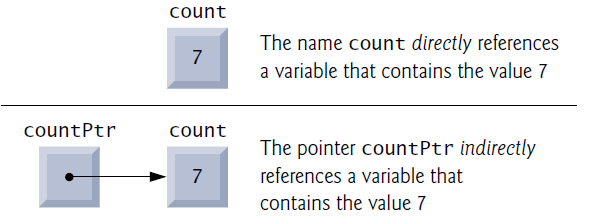
\includegraphics[scale=0.7]{Puntero}
	\end{figure}

	La declaración se da con un asterisco.
	
	\begin{lstlisting}[style=CStyle]
		int *countPtr;
	\end{lstlisting}
	El operador \& sirve para asignar la dirección de una variable.
	\begin{lstlisting}[style=CStyle]
		int y = 5;
		int *yPtr;
		yPtr = &y;
	\end{lstlisting}
\end{frame}

%%%%%%%%%%%%%%%%% FRAME %%%%%%%%%%%%%%%%%%%%%%%%%%
\begin{frame}[fragile]
	\frametitle{Punteros en C}
	El operador $*$ sirve para retornar el valor a donde apunta el puntero. 
	\begin{lstlisting}[style=CStyle]
		printf("\% d, *yPtr");
	\end{lstlisting}
	\vspace{-0.3in}
	\begin{figure}
		\centering
		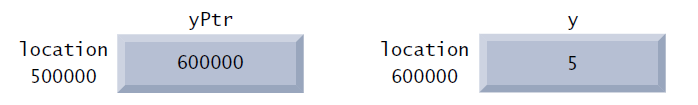
\includegraphics[scale=0.6]{MemoriaPuntero}
	\end{figure}

	\begin{lstlisting}[style=CStyle]
		#include <stdio.h>
		
		int main(void)
		{
			int a = 7;
			int *aPtr = &a; // set aPtr to the address of a
			printf("The address of a is % p"
					"\nThe value of aPtr is % p", &a , aPtr);
			
			printf("\n\nThe value of a is % d"
					"\nThe value of *aPtr is % d", a, *aPtr);
			
			printf("\n\nShowing that * and & are complements of "
					"each other\n&*aPtr = % p"
					"\n*&aPtr = % p\n", &*aPtr, *&aPtr);
		}
	\end{lstlisting}
\end{frame}

%%%%%%%%%%%%%%%%% FRAME %%%%%%%%%%%%%%%%%%%%%%%%%%
\begin{frame}[fragile]
	\frametitle{Pasar argumentos a una función en C}
	En C se pueden usar punteros para pasar valor de una variable a una función. Cuando se realiza este tipo de operación se conoce como paso por referencia ya que se envia la dirección de memoria a modificar. 
	
	\textcolor{blue}{Paso por valor}
	\begin{lstlisting}[style=CStyle]
		#include <stdio.h>
		int cubeByValue(int n); // prototype
		int main(void)
		{
			int number = 5; // initialize number
			printf("The original value of number is %d", number);
			
			// pass number by value to cubeByValue
			number = cubeByValue(number);
			printf("\nThe new value of number is %d\n", number);
		}
		
		// calculate and return cube of integer argument
		int cubeByValue(int n)
		{
			return n * n * n; // cube local variable n and return result
		}
	\end{lstlisting}
\end{frame}

%%%%%%%%%%%%%%%%% FRAME %%%%%%%%%%%%%%%%%%%%%%%%%%
\begin{frame}[fragile]
	\frametitle{Pasar argumentos a una función en C} 
	\textcolor{blue}{Paso por referencia}
	\begin{lstlisting}[style=CStyle]
		#include <stdio.h>
		void cubeByReference(int *nPtr); // function prototype
		
		int main(void)
		{
			int number = 5; // initialize number
			printf("The original value of number is %d", number);
			
			// pass address of number to cubeByReference
			cubeByReference(&number);
			printf("\nThe new value of number is %d\n", number);
		}
		// calculate cube of *nPtr; actually modifies number in main
		void cubeByReference(int *nPtr)
		{
			*nPtr = *nPtr * *nPtr * *nPtr; // cube *nPtr
		}
	\end{lstlisting}
\end{frame}


%%%%%%%%%%%%%%%%% FRAME %%%%%%%%%%%%%%%%%%%%%%%%%%
\begin{frame}[fragile]
	\frametitle{Pasar una cadena}
	\begin{lstlisting}[style=CStyle]
		#include <stdio.h>
		#include <ctype.h>
		void convertToUppercase( char *sPtr ); // prototype
		
		int main(void)
		{
			char string[] = "cHaRaCters and $32.98"; // initialize char array
			
			printf("The string before conversion is: %s", string);
			convertToUppercase(string);
			printf("\nThe string after conversion is: %s\n", string);
		}
		
		// convert string to uppercase letters
		void convertToUppercase( char *sPtr )
		{
			while ( *sPtr != '\0' ) { // current character is not '\0'
				*sPtr = toupper(*sPtr); // convert to uppercase
				++sPtr; // make sPtr point to the next character
			}
		}
	\end{lstlisting}
\end{frame}

%%%%%%%%%%%%%%%%% FRAME %%%%%%%%%%%%%%%%%%%%%%%%%%
\begin{frame}[fragile]
	\frametitle{Usando el identificador \texttt{const}}
	El calificador const es usado para indicar al compilador que dicho valor no va a modificarse. Si una variable no cambia en el cuerpo de una función se debe declarar como constante.
	\begin{multicols}{2}  
		\begin{lstlisting}[style=CStyle]
#include <stdio.h>
void printCharacters( );

int main(void)
{
	// initialize char array
	char string[] = "print characters of a string";
	
	puts("The string is:");
	printCharacters(string);
	puts("");
}

// sPtr is a "read-only" pointer
void printCharacters(const char *sPtr){
	// loop through entire string
	for (; *sPtr != '\0'; ++sPtr) { // no initialization
		printf("%c", *sPtr);
	}
}
		\end{lstlisting}
	\end{multicols}

\textbf{Tarea}: implementar algoritmo de ordenamiento por burbuja utilizando paso por referencia. 
\end{frame}
%%%%%%%%%%%%%%%%% FRAME %%%%%%%%%%%%%%%%%%%%%%%%%%
\begin{frame}[fragile]
	\frametitle{Operador \texttt{sizeof}}
	Es un operador que sirve para determinar el tamaño de bytes de una variable. 
	\begin{lstlisting}[style=CStyle]
	#include <stdio.h>
	#define SIZE 20
	
	size_t getSize(float *ptr); // prototype
	
	int main(void)
	{
		float array[SIZE]; // create array
		
		printf("The number of bytes in the array is % u"
		"\nThe number of bytes returned by getSize is % u\n",
		sizeof(array) , getSize(array) );
	}
	// return size of ptr
	size_t getSize(float *ptr){
		return sizeof(ptr);
	}
	\end{lstlisting}
\end{frame}

%%%%%%%%%%%%%%%%% FRAME %%%%%%%%%%%%%%%%%%%%%%%%%%
\begin{frame}
	\frametitle{Expresiones con punteros}
	Los punteros pueden ser usados para apuntar a los valores de un vector.
	
	\texttt{vPtr = v;}
	
	\texttt{vPtr = \&v[0];}
	
	\begin{figure}
		\centering
		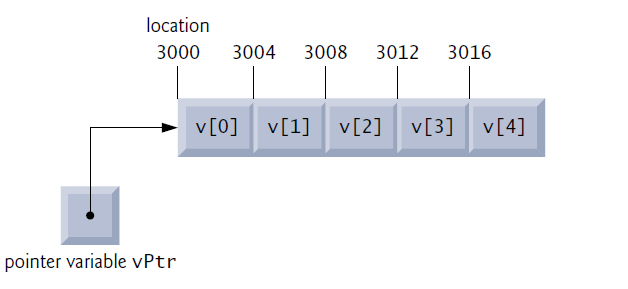
\includegraphics[scale=0.5]{PunteroArreglo}
	\end{figure}

	Al operar con el puntero recuerde que esta operando sobre el valor de la direccion. 
	
	\texttt{vPtr +=2;}
	
	El puntero por lo anterior estara posicionado en \texttt{v[2]}	
\end{frame}

%%%%%%%%%%%%%%%%% FRAME %%%%%%%%%%%%%%%%%%%%%%%%%%
\begin{frame}[fragile]
	\frametitle{Expresiones con punteros - Ejemplo}
	\begin{multicols}{2}
	\begin{lstlisting}[style=CStyle]
#include <stdio.h>
#define ARRAY_SIZE 4

int main(void)
{
	int b[] = {10, 20, 30, 40}; 
	int *bPtr = b; 
	
	// output array b using array index notation
	puts("Array b printed with:\nArray index notation");
	
	// loop through array b
	for (size_t i = 0; i < ARRAY_SIZE; ++i) {
		printf("b[%u] = %d\n", i, b[i]);
	}
	
	// output array b 
	puts("\nPointer/offset notation where\n"
	"the pointer is the array name");
	
	for (size_t offset = 0; offset < ARRAY_SIZE; ++offset) {
		printf("*(b + %u) = %d\n", offset, *(b + offset));
	}
	
	// output array b using bPtr and array index notation
	puts("\nPointer index notation");
	for (size_t i = 0; i < ARRAY_SIZE; ++i) {
		printf("bPtr[%u] = %d\n", i, bPtr[i] );
	}
	
	// output array b 
	puts("\nPointer/offset notation");
	for (size_t offset = 0; offset < ARRAY_SIZE; ++offset) {
		printf("*(bPtr + %u) = %d\n", offset, *(bPtr + offset));
	}
}
\end{lstlisting}
	\end{multicols}

\end{frame}

%%%%%%%%%%%%%%%%% FRAME %%%%%%%%%%%%%%%%%%%%%%%%%%
\begin{frame}
	\frametitle{Encuentre el error}
	\begin{figure}
		\centering
		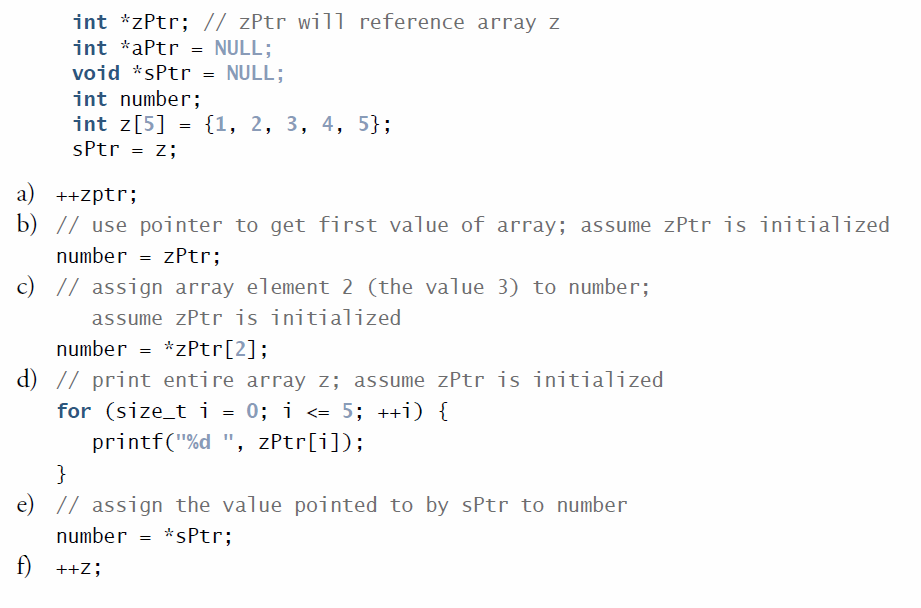
\includegraphics[scale=0.6]{ErrorPuntero}
	\end{figure} 
\end{frame}

%%%%%%%%%%%%%%%%% FRAME %%%%%%%%%%%%%%%%%%%%%%%%%%
\frame{
	\frametitle{Expresiones con punteros}
	\textbf{Ejemplo}: desarrolle un programa que realice operaciones elemento a elementos tales como exponencial.
	
	\textbf{Tarea}: investigue como hacer punteros a funciones y haga un ejemplo. 	
	
	\textbf{Tarea}: implementar un programa en C que baraje y entregue las cartas. Recuerde que una baraja tiene cuatro caras: espadas, corazones, treboles, y diamantes. Cada una de esas son 13 cartas. 
}



%%%%%%%%%%%%%%%%% FRAME %%%%%%%%%%%%%%%%%%%%%%%%%%
\frame{
\begin{center}
	\LARGE \textcolor{blue}{PUNTEROS EN C}
\end{center}

\begin{center}
	\LARGE \textcolor{blue}{GRACIAS}
\end{center}
}

%%%%%%%%%%%%%%%%%%%%%%%%%%%%%%%%%%%%%%%%%%%%%%%%%%%%%%%%%%%%%%%%%%%%%%%%%%%%%%%%%%%%%%%%%%%%%%%%%%%%%%%%%%%%%



\end{document}

